%%%%%%%%%%%%%%%%%%%%%%%%%%%%%%%%%%%%%%%%%%%%%%%%%%%%%%%%%%%%%%%%%%%%%%%%%%%%
%% Author template for Management Science (mnsc) for articles with e-companion (EC)
%% Mirko Janc, Ph.D., INFORMS, mirko.janc@informs.org
%% ver. 0.95, December 2010
%%%%%%%%%%%%%%%%%%%%%%%%%%%%%%%%%%%%%%%%%%%%%%%%%%%%%%%%%%%%%%%%%%%%%%%%%%%%
%\documentclass[mnsc,blindrev]{informs3} % current default for manuscript submission
%\documentclass[mnsc,nonblindrev]{informs3}
\documentclass[msom,blindrev]{informs3}
\OneAndAHalfSpacedXI % current default line spacing
%%\OneAndAHalfSpacedXII
%%\DoubleSpacedXII
%\DoubleSpacedXI

% If hyperref is used, dvi-to-ps driver of choice must be declared as
%   an additional option to the \documentstyle. For example
%\documentclass[dvips,mnsc]{informs3}      % if dvips is used
%\documentclass[dvipsone,mnsc]{informs3}   % if dvipsone is used, etc.

% Private macros here (check that there is no clash with the style)
\usepackage{graphicx}

% Natbib setup for author-year style
\usepackage{natbib}
 \bibpunct[, ]{(}{)}{,}{a}{}{,}%
 \def\bibfont{\small}%
 \def\bibsep{\smallskipamount}%
 \def\bibhang{24pt}%
 \def\newblock{\ }%
 \def\BIBand{and}%

\usepackage{booktabs}

%%package to comment a whole block
\usepackage{verbatim}
%% Setup of theorem styles. Outcomment only one.
%% Preferred default is the first option.
\TheoremsNumberedThrough     % Preferred (Theorem 1, Lemma 1, Theorem 2)
%\TheoremsNumberedByChapter  % (Theorem 1.1, Lema 1.1, Theorem 1.2)
\ECRepeatTheorems

%% Setup of the equation numbering system. Outcomment only one.
%% Preferred default is the first option.
\EquationsNumberedThrough    % Default: (1), (2), ...
%\EquationsNumberedBySection % (1.1), (1.2), ...

% For new submissions, leave this number blank.
% For revisions, input the manuscript number assigned by the on-line
% system along with a suffix ".Rx" where x is the revision number.
\MANUSCRIPTNO{}

%%%%%%%%%%%%%%%%
\begin{document}
%%%%%%%%%%%%%%%%

% Outcomment only when entries are known. Otherwise leave as is and
%   default values will be used.
%\setcounter{page}{1}
%\VOLUME{00}%
%\NO{0}%
%\MONTH{Xxxxx}% (month or a similar seasonal id)
%\YEAR{0000}% e.g., 2005
%\FIRSTPAGE{000}%
%\LASTPAGE{000}%
%\SHORTYEAR{00}% shortened year (two-digit)
%\ISSUE{0000} %
%\LONGFIRSTPAGE{0001} %
%\DOI{10.1287/xxxx.0000.0000}%

% Author's names for the running heads
% Sample depending on the number of authors;
% \RUNAUTHOR{Jones}
% \RUNAUTHOR{Jones and Wilson}
% \RUNAUTHOR{Jones, Miller, and Wilson}
% \RUNAUTHOR{Jones et al.} % for four or more authors
% Enter authors following the given pattern:
%\RUNAUTHOR{}

% Title or shortened title suitable for running heads. Sample:
% \RUNTITLE{Bundling Information Goods of Decreasing Value}
% Enter the (shortened) title:
\RUNTITLE{Customer Reviews in an Online Solar Marketplace}

% Full title. Sample:
% \TITLE{Bundling Information Goods of Decreasing Value}
% Enter the full title:
\TITLE{Customer Reviews in an Online Solar Marketplace}

% Block of authors and their affiliations starts here:
% NOTE: Authors with same affiliation, if the order of authors allows,
%   should be entered in ONE field, separated by a comma.
%   \EMAIL field can be repeated if more than one author
\ARTICLEAUTHORS{%
\AUTHOR{Snidely Slippery}
\AFF{Department of Bread Spread Engineering, Dairy University, Cowtown, IL 60208, \EMAIL{slippery@dairy.edu}} %, \URL{}}
\AUTHOR{Marg Arinella}
\AFF{Institute for Food Adulteration, University of Food Plains, Food Plains, MN 55599, \EMAIL{m.arinella@adult.ufp.edu}}
% Enter all authors
} % end of the block

\ABSTRACT{%
This paper
% Enter your abstract
}%

% Sample
%\KEYWORDS{deterministic inventory theory; infinite linear programming duality;
%  existence of optimal policies; semi-Markov decision process; cyclic schedule}

% Fill in data. If unknown, outcomment the field
\KEYWORDS{marketplace, reviews} \HISTORY{Update: November, 2019}

\maketitle
%%%%%%%%%%%%%%%%%%%%%%%%%%%%%%%%%%%%%%%%%%%%%%%%%%%%%%%%%%%%%%%%%%%%%%

% Samples of sectioning (and labeling) in MNSC
% NOTE: (1) \section and \subsection do NOT end with a period
%       (2) \subsubsection and lower need end punctuation
%       (3) capitalization is as shown (title style).
%
%\section{Introduction.}\label{intro} %%1.
%\subsection{Duality and the Classical EOQ Problem.}\label{class-EOQ} %% 1.1.
%\subsection{Outline.}\label{outline1} %% 1.2.
%\subsubsection{Cyclic Schedules for the General Deterministic SMDP.}
%  \label{cyclic-schedules} %% 1.2.1
%\section{Problem Description.}\label{problemdescription} %% 2.

% Text of your paper here

\section{Introduction}

Solar energy is booming in the U.S. and the rest of the world. It is one of the fastest growing energy generating technology with a dazzling 34\% growth worldwide in 2017 \citep{iea2018snapshot}. More and more, electricity customers have been installing solar panels to generate their own power, reducing the reliance on the electric utilities. This small-scale solar installations skyrocketed in the last decade. Specifically, th


 Solar PV capacity increased by an annual rate of 50\%  in decade and residential solar is forecasted to grow 25\% per year \citep{weaver_2019,seia}; with an even larger upside in the U.S after the passing of California Solar mandate \citep{gtmsolar2018}.
In the U.S., electricity customers have been increasingly installing solar panels to .
Our paper focuses on solar panel  \\


% Just 6\% of American household have already installed solar panels at home with another 46\% say they have given serious thought to adding solar panels at their home in the past year (CITE kennedy thigpen 2019).
 


Online marketplaces is an innovative business model that has shown to ease the rooftop solar panel adoption process. It serves as an intermediary which connects buyers and made the whole process more transparent \citep{dorsey2019access}. There is an increasing trend of installing rooftop panels through online market places. Consumer interest doubled in 11 states between 2017 to 2018, according to an analysis of website traffic \citep{energysageintel19}.  \\

In building an online marketplace, online reviews is considered an essential functionality. Studies have shown that reviews have significant impact on customers'  decision making process, especially for products and services that entail searching and experiencing attributes \citep{zimmermann2018decomposing}.  \\
In the literature, there are papers that show the positive impact of reviews on sales. There are also other papers that demonstrate  (AVERAGE LIT (Literature considered average effect)).\\
In this paper, different from this literature, our primary goal is to study the impact of dispersion of ratings on the  performance metric of the platform, which is a composite of many firms. To the best of our knowledge, there is no prior work that has studied this.

Our paper is also related to papers that investigates the effect of ratings on a single firm's performance metrics. In that stream, there is no consensus about the ultimate impact of dispersion of ratings on the firm's performance metric. Studies have demonstrated positive impacts \citep{chintagunta2010effects,chevalier2006effect,dellarocas2007exploring}, insignificant impact \citep{duan2008online}, and negative impacts in some instances \citep{wang2015user}.

Different from these papers, we took a perspective of the marketplace operator. The marketplace perspective is an important one, especially from the marketplace providers' perspectives. Many new businesses are running a marketplace business model, and have designed the customer ratings functionality an essential part of the platform experience (CITE SOMETHING). In our work, we use the total number of successful proposals on a relevant local market to gauge the health of the marketplace. Total number of success proposals as a performance metric is consistent with common business practices in the investment circle \citep{boris_2018,galston_2017} as it is tied to a marketplace business's valuation. \\

Our objective is to understand the impact of review dispersion on the activity level of each participating supplier on the platform, which has not been studied before. Our study provides insights into the operation of a marketplace and ties reviews to


----[OLD VERSION]

Solar cells, also called photovoltaic cells, convert sunlight directly into electricity without carbon emissions. Today, electricity from solar cells has become competitive in many regions and photovoltaic systems are being deployed at large scales to help power the electric grid \citep{nrel.gov}.

Solar energy is blooming in the US and the world. It is one of the fastest growing energy generating technology with a dazzling 34\% growth worldwide in 2017 \citep{iea2018snapshot}. Just 6\% of American household have already installed solar panels at home with another 46\% say they have given serious thought to adding solar panels at their home in the past year (CITE kennedy thigpen 2019).Solar PV capacity increased by an annual rate of 50\%  in decade and residential solar is forecasted to grow 25\% per year \citep{weaver_2019,seia}; with an even larger upside in the U.S after the passing of California Solar mandate \citep{gtmsolar2018}. \\
Online marketplaces is an innovative business model that has shown to ease the rooftop solar panel adoption process. It serves as an intermediary which connects buyers and made the whole process more transparent \citep{dorsey2019access}. There is an increasing trend of installing rooftop panels through online market places. Consumer interest doubled in 11 states between 2017 to 2018, according to an analysis of website traffic \citep{energysageintel19}.  \\
In building an online marketplace, online reviews is considered an essential functionality. Studies have shown that reviews have significant impact on customers'  decision making process, especially for products and services that entail searching and experiencing attributes \citep{zimmermann2018decomposing}.  \\
In the literature, there are papers that show the positive impact of reviews on sales. There are also other papers that demonstrate  (AVERAGE LIT (Literature considered average effect)).\\
In this paper, different from this literature, our primary goal is to study the impact of dispersion of ratings on the  performance metric of the platform, which is a composite of many firms. To the best of our knowledge, there is no prior work that has studied this.

Our paper is also related to papers that investigates the effect of ratings on a single firm's performance metrics. In that stream, there is no consensus about the ultimate impact of dispersion of ratings on the firm's performance metric. Studies have demonstrated positive impacts \citep{chintagunta2010effects,chevalier2006effect,dellarocas2007exploring}, insignificant impact \citep{duan2008online}, and negative impacts in some instances \citep{wang2015user}.

Different from these papers, we took a perspective of the marketplace operator. The marketplace perspective is an important one, especially from the marketplace providers' perspectives. Many new businesses are running a marketplace business model, and have designed the customer ratings functionality an essential part of the platform experience (CITE SOMETHING). In our work, we use the total number of successful proposals on a relevant local market to gauge the health of the marketplace. Total number of success proposals as a performance metric is consistent with common business practices in the investment circle \citep{boris_2018,galston_2017} as it is tied to a marketplace business's valuation. \\

Our objective is to understand the impact of review dispersion on the activity level of each participating supplier on the platform, which has not been studied before. Our study provides insights into the operation of a marketplace and ties reviews to



\section{How Reviews Dispersion Impacts Activity Intensity(Literature Review) }
 In this section we describe several mechanisms by which reviews dispersion may impact installers activity intensity on a platform.


\section{Data and Setting}

We analyze the interplay between customer reviews and firm activities (and outcomes) in an online marketplace for electricity end-users' solar panel installations. To do so, we collaborated with an online solar marketplace company, and obtained the full record of customer reviews and installer actions on a monthly level from 2013 to 2018 in the marketplace. This data set is proprietary and the primary source of our analysis. We also complement the marketplace data with Tracking The Sun (TTS) data set from the Lawrence Berkeley National Laboratory. TTS is a comprehensive publicly available data set about U.S. solar panel installations. Below, we provide details about the setting of the online solar marketplace we study and our data.


%We use a compilation of proprietary and publicly available data about residential solar markets. The focus of the study is about the actions and outcomes of an online marketplace for residential solar installations. We obtained, via collaboration with the marketplace company, the full record of customer reviews and installer actions on a monthly level from 2013 to 2018. We complement the marketplace data with Tracking The Sun (TTS) data set from Lawrence Berkeley National Laboratory. TTS aggregates data from more than 60 state and utility incentive programs. The full TTS data set covers more than 80\% of the U.S. PV
%market, making it the most comprehensive extant U.S. PV data set. It contains installation level information such as installer name, unit size and price which allow us to construct a big picture of solar installation activities that are happening on and off the marketplace. 

\subsection{Online Solar Marketplace}
The solar marketplace (MKT) is an independent shopping website for electricity end-users, i.e., customers. It lets solar panel installers maintain a profile and receive potential customer information. Here is how it operates. First, each customer visits the marketplace website and enters her information, such as the location of her property. Second, the marketplace informs all installers about the arrival of the customer along with her information. Every installer that provides service to the customer's location decide whether to make a proposal (\emph{bid}) to the customer. After the customer observes installer proposals, there are two possible outcomes: Either the customer agrees with an installer, i.e., there is a successful match, or the customer gives up the process, i.e., there is no matching.


[PLEASE READ THIS SENTENCE AND VERIFY THE CORRECTNESS]In this context, we obtained rich panel data from the solar marketplace that contain all its vetted installers, installers' monthly actions and performance (i.e., number of bids made and number of bids won) and all customer reviews (text content and ratings) from the beginning of the platform up to April of 2018.

\subsection{Installers}
The actions of solar installers is the focus of our study. Through communicating with the online marketplace company, we learned that the Solar Installers decision on the platform are as follows:

\begin{enumerate}
\item  \textbf{Join}. Join the platform. We have been told that the marketplace actively reach out to solar installers to recruit them to join to platform and help them set up the website. So unlike physical businesses, the fixed cost of entry is minimal for online marketplace \citep{haddad2015consumer}. In this study we do not study the entry of the platform, rather than focusing on installer actions after they have established a profile.  \\
\item  \textbf{Active and put in efforts}. Actively monitor the platform and make proposals to attract potential customers. We are interested in the\textit{ intensity of efforts}, which is measured by how many proposals that an installer makes per month. (FIND REFERENCE THAT THIS TAKES TIME AND EFFORT; IS THE ESSENTIAL DECISION)\\
\end{enumerate}

Lastly, we don't observe quitting the platform the same way as physical store closes off. We simply observe inactive profiles. Thus we do not explicitly investigate the exit behavior. (REMEMBER to ADD ROBUSTNESS CHECK EXCLUDING INACTIVE FIRMS)


\subsection{Ratings and Reviews}
Customers participate on the MKT platform by providing information about their property details for a solar installation. They will then receive installer proposals. If the customer ended up working with the installer, they will have an opportunity to leave a review with ratings range from 1 to 5 stars. The platform verifies the customer who left reviews. Hence, we can treat reviews as authentic and not manipulated. In figure \ref{reviews_example} we provided an example of how reviews information are displayed on the platform.
\begin{figure}
	\centering
	
\includegraphics[width=0.81\linewidth]{reviews_example.png}
	\caption{Reviews Example}
	\label{reviews_example}
\end{figure}


\subsection{Defining Local Market}
\label{defining_local_market}
Solar installers are largely competing on a number of local markets with adjacent installers.  This is characteristic to the residential solar business: solar installation is a combination of product and service; the service component requires installers' multiple visits to the customer site;  customers tend to only seek out local installers and installers tend to only compete locally. This is also reflected in MKT's setting - installers specify a service region; installers will only be notified of customer arrival and act on the lead if the customer falls into that region. Customer also sees installer's distance to their locations and might factor that in their decision. Thus, we want to create a distance and density based \textit{clustering} which reflect the local competition. We shall divide installers into multiple clusters and treat one cluster as one local market. Clustering installers also provides \textbf{identification}. By leveraging the local market level differences in reviews dispersion and local market outcome, we can quantify the impact of reviews dispersion. \\

We do not want to use state, county, or congressional district boarder because it is common for installers to cross these artificial lines to serve customers. Instead, we create local market geographic division with the following steps:
\begin{enumerate}
	\item For every MKT installer, we determine its location using the 5-digit zip code they listed. We use the representative coordinates of that Zipcode based on data provided by the US Census(https://www.census.gov/geo/maps-data/data/gazetteer.html).
	\item  We run a location and density based clustering algorithm(OPTICS, more details below) to cluster the pool of installers' coordinates. We later refer to the clusters generated as "markets".  Ordering points to identify the clustering structure (OPTICS) is an algorithm for finding density-based clusters in spatial data. (PROVIDE A BIT MORE INFO , WHO USED IT, ETC).
	\item OPTICS is an unsupervised machine learning algorithm. In order to determine the optimal combination of parameters, we ran a grid search for its critical parameter inputs - radius - from 10 miles to 150 miles and used Calinski-Harabasz index as benchmark. We settled on the radius at 90 miles to be optimal and arrived at 36 clusters, each cluster contains X to X installers. We use this cluster to define our market boundary geographically. (PROVIDE A PICTURE TO ILLUSTRATE THE CALINSKI-HARABASZ CURVE VS PARAMETER)
\end{enumerate}
The figures \ref{fig:nationalinstallers} and \ref{fig:markets} illustrated the process of allocating geographically dispersed installers (first figure) into clusters, with the centroid of each cluster marked in the second figure representing local markets.
\begin{figure}
	\centering
	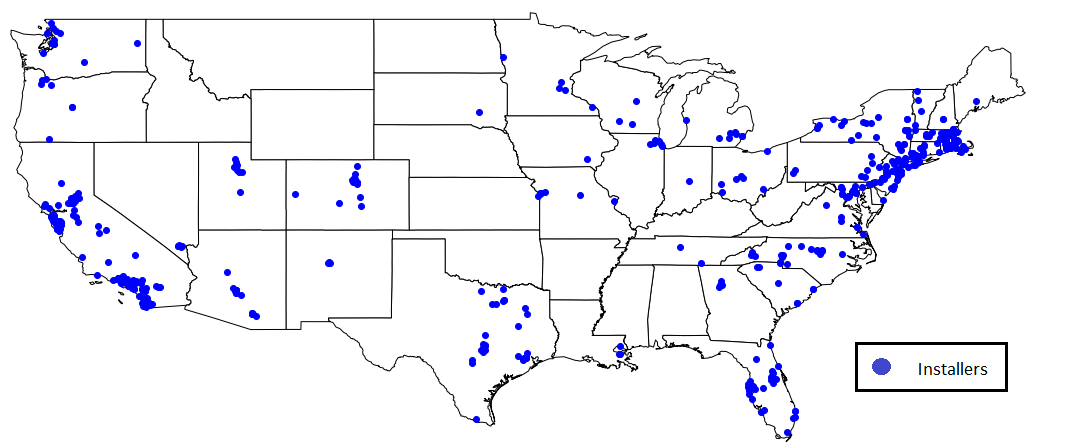
\includegraphics[width=1.1\linewidth]{national_installers.png}
	\caption{All Installers}
	\label{fig:nationalinstallers}
\end{figure}
\begin{figure}
	\centering
	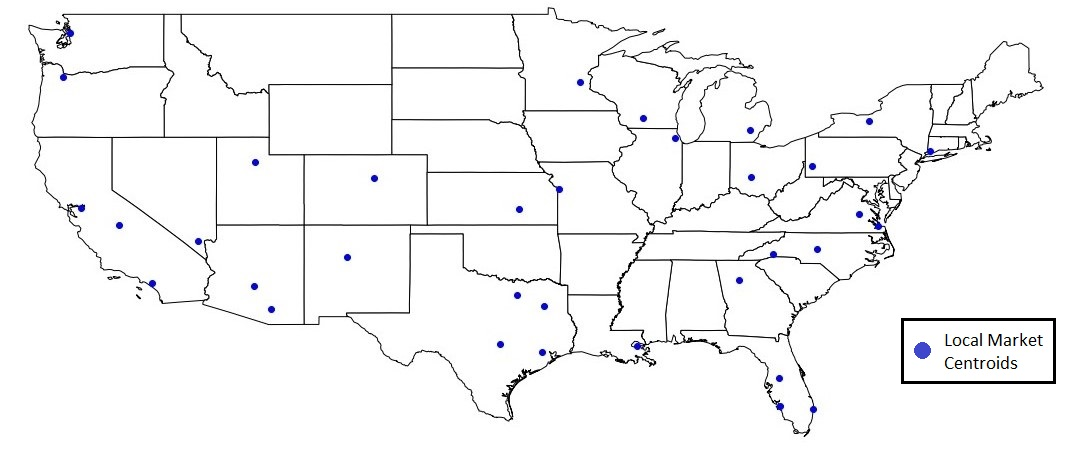
\includegraphics[width=1.1\linewidth]{markets.jpg}
	\caption{Local Market Centroids}
	\label{fig:markets}
\end{figure}


\section{Model and Measures}
In this section we describe our empirical methods. First we introduce the key dependent variable - dispersion of the reviews. We constructed two sets of variables to measure the dispersion of the reviews with both the numeric rating and the reviews text. We first quantify the impact of dispersion with the activity intensity on an individual installer level; we then elevate our analysis to the platform level by connecting the impact of dispersion on local market level total transactions in relation to the dispersion in reviews.

\subsection{Measure Reviews Dispersion}
\label{subsection_measure_dispersion}
We are first interested in measuring the dispersion in ratings, i.e, the quantitative information provided by the ratings. Customer leave a piece of reviews after their solar installation experience. The reviews is composed of a rating ( from 1 to 5 stars) and a piece of texts. We first discribe how we measure reviews dispersion from the quantitative ratings information. We also introduce an innovative word embedding model that measures reviews dispersion from the texts data.
\subsubsection{Capture Dispersion in Numeric Ratings}
We use the concept of entropy to capture dispersion in ratings and to construct the independent variable of interests to capture the dispersion of ratings. Entropy is a common measure in information theory (ADD ONE MORE sentence to explain). It can be applied to a collection of a set of discrete probabilistic outcomes, which is our case is the discrete number of ratings ( from 1 to 5) that each piece of reviews receive. \\
The formula of computing entropy on a set of discrete values is:  \\
\begin{equation}
H(X)=-\sum P(X)log(1/P(x)))
\end{equation}
For example, we want to measure the ratings dispersion on a set of 5 reviews, they all got 4-stars (out of 5). Therefore, we will be applying the calculation on a set $\{4,4,4,4,4\}$. Following the formula, this set of reviews has an entropy of 0. Alternatively, if we have a set of reviews as $\{3,5,3,5,4\}$, the entropy of this set of reviews is 1.0549.  Although both have the same average rating (4), the second set of ratings are more informative with a higher dispersion, hence has a higher entropy measure. \\

We apply the entropy calculation on the dataset. For every installer-month, we calculate the ratings entropy on three scopes: \\
1. Entropy on own reviews, denote as $ENT_{self,i,t}$. This is calculated on the set of reviews that are associated with the focal installer $i$ up to month $t$.  \\
2. Entropy on peer installers' reviews, up to that month, denote as $ENT_{others,i,t}$. This is calculated on the set of reviews that are associated with all the other installers on focal installer's local market, per market boundaries that were set following steps described in \ref{defining_local_market}.  \\
We also calculate entropy on the local market level:\\
3. Entropy of all reviews on a local market $m$, up to that month $t$, which we later denote as $ENT_{mkt,m,t}$. This is calculated on a market-month level data set with market defined in \ref{defining_local_market}. \\
Another candidate of measuring dispersion would be the coefficient of variation (CV). Entropy is superior to CV because ratings are far from being normally distributed. Moreover, entropy measure is significantly correlated with CV but are stretched 'longer', reflecting the fact that entropy is the finer measure. We illustrate this point via a scatter plot of CV and Entropy measures \ref{scatter_cv_ent_others}.
\begin{figure}
	\centering
	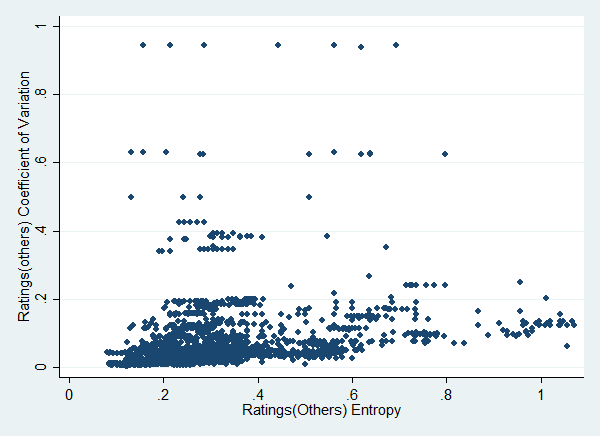
\includegraphics[width=0.7\linewidth]{scatter_cv_ent_others.png}
	\caption{Scatter Plot between CV and Ent measures}
	\label{scatter_cv_ent_others}
\end{figure}

\subsubsection{Capture Dispersion in Texts with Word Embedding model BERT}

In addition to ratings, We want to leverage the rich information in the reviews texts. We hypothesize that the \textit{dispersion} in reviews texts shall also exhibit similar effect as the ratings as well as positively correlated with the entropy. A set of all 5 star reviews with praises might contain less information than a mix of 1, 2 and 5 stars. This is reflected in entropy as the later will have a higher entropy. We aim to design a measure that captures a similar concepts on texts. To achieve that goal of measuring reviews dispersions in texts,  we combine the methods inspired by \cite{hoberg2016text}, tweak it to apply to our data structure,  and updated it with a word embedding model called BERT , which we will describe later. \\
Hoberg and Phillips' work involves measuring the similarity between two pieces of texts. In their case, they measure the distance of the two pieces of business descriptions from 10-k form and take $1 - distance$ to represent similarities between two business entities. Their methods include: 1) Vectorize each piece of text based on the distinct words it contains. 2) Normalize the vectors to unit length. and 3) Use the Cosine similarity to measure how similar are two word vectors. It is called cosine similarity because it measures the angle between the two vectors that represents the texts. If the angle is $0$, their similarity shall be $1$ and distance be $0$. The cosine similarity between the two vectors is calculated as follows: \\
\begin{itemize}
\item Cosine \textit{Similarity} between $V_{1}$ and $V{2} =(V_1 \cdot V_2)$
\item Cosine \textit{Distance} between $V_{1}$ and $V{2}=1-(V_1 \cdot V_2)$
\end{itemize}
We incorporate the aforementioned cosine distance concept to measure dispersion in sets of reviews texts. It is achieved by enumerating all pairwise distances of reviews and take its statistical median. For example, on a set of 10 reviews texts pieces, we have 45 (45=$\binom{10}{2}$) pair-wise distances.  We then compute the median distances of these 45 similarity scores, denoted as $TD$ to represent the \textbf{Text Dispersion}. If the 10 pieces of texts are dissimilar from each other, they contain richer information and the median of these $45$ distances data shall be higher; and vice versa.  \\
Similar to ratings entropy, we compute text-based dispersion on 3 different scopes and use them as Independent Variables of interest: \\

\begin{itemize}
\item 1. Text-based Dispersion for one's own reviews up to month $t$ is computed on the $N_{it}$ reviews available up to month $t$. It is calculated by computing the $N_{it}\times (N_{it}-1)/2$ cosine distance pairs and take the 50 percentile, which is denote as $TD_{self,i,t}$ (TD: Text-based Dispersion)\\
\item 2. Text-based Dispersion for others' review up to month $t$ is computed on the $N_{i,others,t}$ reviews available up to month $t$ that is in focal installer $i$'s local market. It is calculated by computing the $N_{i,others,t}\times (N_{i,others,t}-1)/2$ cosine distance pairs and take the 50 percentile, which is denote as $TD_{Others,i,t}$ \\
\end{itemize}
We also compute the text-based dispersion for every \textit{market-month}: \\

\begin{itemize}
\item 3. Text-based Dispersion for a market $m$ at month $t$ is computed on the $N_{m,t}$ reviews available up to month $t$. Take the  $N_{mt}\times (N_{mt}-1)/2$ cosine distance pairs and take the 50 percentile and denote it as $TD_{market,i,t}$ \\
\end{itemize}

We now describe the process we took to \textit{vectorize} the review texts. In our study, we used a BERT word embedding model \citep{devlin2018bert}. BERT is short for Bidirectioanl Encoder Representations from Transformers (BERT). It is a natural language processing model that transforms texts into numeric vectors while also preserve the semantic meaning of the texts. It is getting widely applied in research and industry application such as Google Search. It belongs to the category of NLP methods called word embedding. We perform word embedding on the texts before computing distance. \\
Some earlier literature such as \cite{hoberg2016text} used simple word counter vectors or combined with a tf-idf (term-frequency-inverse document frequency) weighting scheme in \cite{loughran2011liability}. It was an appropriate application for formal financial documents such as 10-K forms. In our application, we are dealing with texts that are informal writings and often with emotions expressed in the text. Simply capturing word frequencies will not be enough if similar emotions can be expressed with synonymous words. We want to produce vectors that will preserve the information and sentiment of the reviews texts despite use of synonyms and/or different styles. For example, consider 3 sentences: \\
Sentence 1: they did a good job. \\
Sentence 2: they did an awful job. \\
Sentence 3: they did a great job. \\
We want the distance between sentence 1 and 3 to be closer than the distance between 2 and 3 or 1 and 2. Word embedding method enables just that. Word embedding will project "good" and "great" to vectors that are closer together. Without word embedding, the distance between the 3 sentences will be similar ( with tf-idf weighting) or the same ( without tf-idf weighting, simply use a counter vectorizer). \\
Under the BERT model vectorization, \\
Similarity between sentence 1 and 2: 0.9134093016230975\\
Similarity between sentence 2 and 3: 0.9053232267859165\\
Similarity between sentence 1 and 3: 0.9737446020998256\\

We used the python library via spaCy v2.1 to implement BERT. We converted every piece of reviews text, regardless of its original length, into a numeric vector of shape 768 $\times$ 1,  performed calculation on pairwise cosine distances and derived statistical means for every installer-month or market-market as previous mented. The end result is a set of variables representing the dispersion in texts, denoted as $TD_{self,i,t},TD_{Others,i,t},TD_{market,m,t}$ that are parallel to the Entropy measures $ENT_{self,i,t},ENT_{Others,i,t},ENT_{m,t}$ \\


\subsection{Installer Level Analysis}
We aim to find the connection between ratings dispersion on installer activity intensities. The available data were used to construct a panel data set where the unit of analysis is the the measure of activity intensities ($\log$ (proposals generated + 1)) of a particular installer at a specific local market during a month. We use a regression model with fixed effects and clustered the standard errors on the local market level ( individual level yield similar results). We describe our regression models next. \\
Using the indexes $i$ for installer, $m$ for local market, and $t$ for month, the following regression equation is used to estimate the impact of ratings dispersion (own ratings dispersion: $Ent_{i,self,t}$ ; others ratings dispersion: $Ent_{i,others,t}$) on focal installer's activity intensities $ActInt_{i,m,t}$:
\begin{equation}
    ActInt_{im,t+1}=\beta_{0}+\beta_{11} Ent_{im,others,t}+\beta_{2}Ent_{im,others,t}^2+
   Controls_{it}+\alpha_{i}+\epsilon_{imt}
   \label{model_ind_1}
\end{equation}

\begin{equation}
    ActInt_{im,t+1}=\beta_{3}+\beta_{4} Ent_{i,self,t}+\beta_{5}Ent_{i,self,t}^2+
   Controls_{it}+\alpha_{i}+\epsilon_{imt}
   \label{model_ind_2}
\end{equation}

\begin{equation}
    ActInt_{im,t+1}=\beta_{6}+\beta_{7}Ent_{i,self,t}+\beta_{8}Ent_{i,self,t}^2+\beta_{9}Ent_{im,others}+\beta_{10}Ent_{im,self,t}^2+Controls_{it}+\alpha_{i}+\epsilon_{imt}
   \label{model_ind_3}
\end{equation}
 The error term $\epsilon$ represents factors that affect installer activity intensity that are unobservables in the data. $\alpha_{i}$ represents the installer level fixed effects. $Controls_{it}$ are all other installer-level or market level control variables we include in order to capture factors that are irrelevant to reviews dispersion. We detail our selection of control variables next.
\subsubsection{Control Variables}\hfill\\
\textbf{State}: State dummies are included to account for state level policy effects. (ELABORATE)\\
\textbf{Price}: price is an important factor. Although we do not model installers' pricing strategy, we want to control for the impact of price on installers' activities. We decide to look at the price difference between the focal installer and the others. We use Tracking the Sun data to find the installers' prices via matching name and Zipcode. We also use the unit price: price per KW. Price per KW is a common way to assess the price level of a solar system, as the final price tag of the solar system will be dependent on the size. We then compute the variable $PriceDiff_{i,t}$ as the difference in unit price between installer and the average unit price of their competitors on the local market. \\
\textbf{Average Ratings}: the average ratings of installer themselves $avg_{i,t}$ and the average ratings of their competitors $avg_{others,t}$ on the market. \\
\textbf{Experience}: the number of years the installer has been installing solar systems. We obtain that information from installers' website. \\
\textbf{Local Markets Condition} Once the algorithm gave us the clusters that defines market divisions, we augment the data with Tracking The Sun data to capture local market conditions. We use the same Market definition from \ref{defining_local_market} and computed the sum of all solar installations within a market during a month, denote as $MarketRev_{mt}$. The market revenue variable measures the total opportunities of solar installations on that market. \\
In addition, installer level fixed-effects are included to control for time-invariant characteristics of each installers.

\subsection{Market Level Analysis}
We next perform the analysis on a market level. We analyze the connection between market level ratings dispersion and the market level outcomes.  We use a regression model with fixed effects and clustered standard errors on the local market level. \\
To measure the success of the market, we use the total number of accepted quotes. There are several reasons that we use accepted quotes as the performance metrics: 1. The goal of the market place is to help customers connect with installers. 2. The market itself, just like many other market place, is also evaluated by the transaction volume in a business sense. \\
We create the dependent variable of interests using the following data transformation. For every local market $m$, we sum up the total number of quotes accepted per that month ($QuotesWon_{imt}$) for every installers $i$ on that market, and take the log transform.
\begin{align*}
SumQuotes_{m,t}=\sum_{i\in m} QuotesWon_{i,m,t}\\
MarketActivity_{m,t}=\log (SumQuotes_{m,t}+1)
\end{align*}
By doing that, we convert the installer-monthly level panel data from previous section to a market-monthly level panel data so that we can exploit the variations on market level reviews dispersion to identify their impact on local market outcomes.  \\
Using the indexes $m$ for local market, $t$ for month, the following regression equation is used to estimate the impact of ratings dispersion on the local market on the local market performance metrics.
\begin{equation}
    MarketActivity_{m,t+1}=\beta Ent_{m,t}+\beta Ent_{m,t}^2+Controls+\epsilon_{mt}
\end{equation}

Where $MarketActivity_{m,t+1}$ indicate the log of the total number of proposals accepted on market $m$ in month $t+1$, and the model link it to the $Ent_{i,m,t}$ - Entropy of reviews from all installers on that local market.


\subsubsection{Control Variables}\hfill\\
We use the following control variables for the market level analysis\\
\textbf{State}. There are 33 different state represented in the data set, so we created 33 state dummies. Some market span across more than one state. In that case, we weighted state dummy with the percentage. \\
\textbf{Market condition}:
Similar to individual analysis, we use the total monthly revenues from that market to control for market conditions.
\begin{align*}
\log ZipRev_{m,t}=\log \sum_{j\in m}Rev_{j,t}
\end{align*}
 \textbf{The total number of reviews on the market } We use
\begin{align*}
SumReviews_{m,t}=\sum_{i\in m} Reviews_{i,m,t}
\end{align*}


\section{Results}
We now presetn the results of our analysis.
\subsection{Summary Statistics}
In the merged data set, we have a installer-month level panel data set that depicted installers' actions. The data set features:
\begin{itemize}
\item Solar installers: 416 different installers
\item Time period: from 2013 to 2018
\item Ratings and reviews: 3607 pieces of review records with the rating, text content, timestamp, and the installer with which each review is associated
\end{itemize}
Our final sample consisted of 416 individual installers on the market place, 3607 pieces of reviews records with rating, texts content and time stamp. In table \ref{sumstats_ind} and \ref{corr_ind}, we present the descriptive statistics and correlation matrix for the independent and dependent variables on individual installer level.  In table \ref{sumstats_mkt} and \ref{corr_mkt} we present that on the local market level. We find that the correlations are generally in the expected direction and not a huge concern for the validity of regression analysis.
% Please add the following required packages to your document preamble:
% \usepackage{booktabs}
% \usepackage{graphicx}
\begin{table}[H]
\centering
\begin{tabular}{@{}lccccc@{}}
\toprule
Variables               & N     & Mean    & Standard Deviation & Min    & Max   \\ \midrule
Rating\_Entropy\_Self   & 4,562 & 0  & 0.217  & -0.0985 & 0.9015     \\
Rating\_Entropy\_Others & 4,562 & 0   & 0.183  & -0.227  & 0.773     \\
Average\_Rating\_Self   & 4,562 & 4.531   & 1.316  & 1      & 5     \\
Average\_Rating\_Others & 4,562 & 4.88    & 0.205  & 1      & 5     \\
Review\_Count           & 4,562 & 5.384   & 6.836  & 0      & 52    \\
Experience              & 4,562 & 1.758   & 0.929  & 0      & 3.714 \\
Price\_Difference       & 4,562 & -0.0333 & 0.392  & -2.171 & 3.139 \\
Market\_LogRevenue      & 4,562 & 12.24   & 7.9    & 0      & 22.3  \\ \bottomrule
\end{tabular}%
\caption{Summary Statistics - Installer Level Analysis}
\label{sumstats_ind}
{\footnotesize \textit{Note: All entropy variables are demeaned.}}
\end{table} 
% Please add the following required packages to your document preamble:
% \usepackage{booktabs}
\begin{table}
\centering
\begin{tabular}{@{}llllll@{}}
\toprule
               & Obs & Mean     & SD       & Min & Max      \\ \midrule
Installations  & 791 & 3.978508 & 8.775443 & 0   & 91       \\
Reviews(Mkt)   & 791 & 28.90771 & 47.33097 & 0   & 314      \\
Ratings(Mkt)   & 773 & 4.872664 & .2431345 & 3   & 5        \\
Entropy        & 791 & .184022  & .2330093 & 0   & 1.05492  \\
Market Revenue & 791 & 7.906193 & 8.114449 & 0   & 22.30267 \\ \bottomrule
\end{tabular}
\caption{Summary Statistics Market Level}
\label{sumstats_mkt}
\end{table}

% Please add the following required packages to your document preamble:
% \usepackage{booktabs}
\begin{table}
\centering
\begin{tabular}{@{}lccccccc@{}}
\toprule
 & \multicolumn{1}{l}{Reviews Ct} & \multicolumn{1}{l}{Ent(Self)} & \multicolumn{1}{l}{Ent(Others)} & \multicolumn{1}{l}{Ent(Market)} & \multicolumn{1}{l}{Exp} & \multicolumn{1}{l}{Price} & \multicolumn{1}{l}{Mkt Rev} \\ \midrule
Reviews Count & 1 &  &  &  &  &  &  \\
Entropy(Self) & 0.252 & 1 &  &  &  &  &  \\
Entropy(Others) & 0.077 & -0.044 & 1 &  &  &  &  \\
Entropy(Market) & 0.089 & 0.321 & 0.823 & 1 &  &  &  \\
Experience(Log) & 0.171 & 0.017 & 0.093 & 0.104 & 1 &  &  \\
Price(Diff) & -0.044 & -0.006 & -0.030 & -0.01 & -0.008 & 1 &  \\
Local Market Revenue(Log) & -0.037 & -0.032 & -0.041 & -0.058 & 0.637 & -0.034 & 1 \\ \bottomrule
\end{tabular}
\caption{Correlation Individual Level}
\label{corr_ind}
\end{table}
% Please add the following required packages to your document preamble:
% \usepackage{booktabs}
\begin{table}
\centering
\begin{tabular}{@{}llllll@{}}
\toprule
 & Instal& Reviews Ct & Ratings & Ent(Mkt) & Mkt Rev \\ \midrule
Installations(Mkt, log) & 1.000 &  &  &  &  \\
Reviews(Mkt, Log) & 0.731 & 1.000 &  &  &  \\
Average Reviews(Mkt) & -0.013 & -0.020 & 1.000 &  &  \\
Entropy(Mkt) & 0.228 & 0.306 & -0.572 & 1.000 &  \\
Mkt Rev(Log) & 0.345 & 0.228 & -0.032 & 0.158 & 1.000 \\ \bottomrule
\end{tabular}
\caption{Correlation Market Level}
\label{corr_mkt}
\end{table}

\subsection{Individual Installer}
%% Please add the following required packages to your document preamble:
% \usepackage{booktabs}
\begin{table}
\centering
\begin{tabular}{@{}lllll@{}}
\toprule
 & (1) & (2) & (3) & (4) \\ \midrule
 & F.Activity & F.Activity & F.Activity & F.Activity \\
Avg & -0.655 & -0.655 & -0.333 & -0.333 \\
 & (0.345) & (0.283) & (0.612) & (0.605) \\
Avg \# Avg & 0.0471 & 0.0471 & 0.00302 & 0.00302 \\
 & (0.660) & (0.614) & (0.976) & (0.974) \\
Reviews Count & 0.0480* & 0.0480* & 0.0492* & 0.0492* \\
 & (0.000) & (0.000) & (0.000) & (0.000) \\
Avg(Others) & -0.0285 & -0.0285 & -0.0453 & -0.0453 \\
 & (0.873) & (0.876) & (0.812) & (0.800) \\
Entropy Others  & 1.762* & 1.762* & 1.918* & 1.918* \\
 & (0.020) & (0.012) & (0.006) & (0.003) \\
Experience & 0.212* & 0.212* & 0.191* & 0.191* \\
 & (0.021) & (0.018) & (0.005) & (0.009) \\
Price Diff & 0.0861 & 0.0861 & 0.000934 & 0.000934 \\
 & (0.569) & (0.557) & (0.994) & (0.995) \\
Market Revenue & -0.0169+ & -0.0169* & -0.0171+ & -0.0171* \\
 & (0.074) & (0.023) & (0.066) & (0.015) \\
Entropy Others  \# Entropy Others  & -2.626* & -2.626* & -2.704* & -2.704* \\
 & (0.001) & (0.005) & (0.000) & (0.002) \\
Constant & 4.062* & 4.062* & 4.389* & 4.389* \\
 & (0.004) & (0.004) & (0.002) & (0.004) \\
Observations & 4190 & 4190 & 4190 & 4190 \\ 
\bottomrule
\end{tabular}
\caption{Individual Level Regression Results}
\label{table_regression_ind}
\end{table}
% Please add the following required packages to your document preamble:
% \usepackage{booktabs}
% \usepackage{graphicx}
\begin{table}
\centering
\resizebox{\textwidth}{!}{%
\begin{tabular}{@{}lcccc@{}}
\toprule
 & (1) & (2) & (3) & (4) \\ \midrule
 & F.Activity & F.Activity & F.Activity & F.Activity \\
Avg & -1.170+ & -1.170* & -1.155+ & -1.155* \\
 & (0.068) & (0.043) & (0.060) & (0.042) \\
Avg \# Avg & 0.130 & 0.130 & 0.129 & 0.129 \\
 & (0.180) & (0.134) & (0.170) & (0.132) \\
Reviews Count & 0.0452* & 0.0452* & 0.0423* & 0.0423* \\
 & (0.000) & (0.000) & (0.000) & (0.000) \\
Avg(Others) & -0.0310 & -0.0310 & -0.0273 & -0.0273 \\
 & (0.857) & (0.839) & (0.887) & (0.884) \\
Experience & 0.211* & 0.211* & 0.207* & 0.207* \\
 & (0.019) & (0.018) & (0.023) & (0.018) \\
Price Diff & 0.0863 & 0.0863 & 0.0928 & 0.0928 \\
 & (0.554) & (0.529) & (0.516) & (0.512) \\
Market Revenue & -0.0163 & -0.0163* & -0.0160 & -0.0160* \\
 & (0.107) & (0.031) & (0.109) & (0.034) \\
Entropy Own & 2.616* & 2.616* & 2.676* & 2.676* \\
 & (0.006) & (0.007) & (0.004) & (0.005) \\
Entropy Own \# Entropy Own & -3.090* & -3.090* & -3.301* & -3.301* \\
 & (0.042) & (0.025) & (0.020) & (0.015) \\
Entropy Others &  &  & 1.740* & 1.740* \\
 &  &  & (0.022) & (0.011) \\
Entropy Others \# Entropy Others &  &  & -2.674* & -2.674* \\
 &  &  & (0.001) & (0.003) \\
Constant & 4.698* & 4.698* & 4.519* & 4.519* \\
 & (0.001) & (0.000) & (0.002) & (0.002) \\
Observations & 4190 & 4190 & 4190 & 4190 \\
p-values in parentheses &  &  &  &  \\
="+ p\textless{}0.10 & * p\textless{}0.05" &  &  &  \\ \bottomrule
\end{tabular}%
}
\caption{Regression with Own Entropy}
\label{table_regression_ind_withentself}
\end{table}
% Please add the following required packages to your document preamble:
% \usepackage{booktabs}
\begin{table}
\centering
\begin{tabular}{@{}lcccccc@{}}
\toprule
 & (1) & (2) & (3) & (4) & (5) & (6) \\ \midrule
 & F.Activity & F.Activity & F.Activity & F.Activity & F.Activity & F.Activity \\
Avg & -0.655 & -0.623 & -0.689 & -0.850+ & -0.966* & -1.188* \\
 & (0.345) & (0.393) & (0.327) & (0.055) & (0.032) & (0.016) \\
Avg \# Avg & 0.0471 & 0.0660 & 0.0521 & 0.0926 & 0.122+ & 0.154* \\
 & (0.660) & (0.566) & (0.632) & (0.207) & (0.085) & (0.038) \\
Reviews Count & 0.0480* & 0.0483* & 0.0441* & 0.0230* & 0.0268* & 0.0229* \\
 & (0.000) & (0.001) & (0.000) & (0.002) & (0.001) & (0.002) \\
Avg(Others) & -0.0285 & -0.0838 & -0.0550 & -0.0435 & -0.107 & -0.0643 \\
 & (0.873) & (0.651) & (0.760) & (0.795) & (0.486) & (0.731) \\
Experience & 0.212* & 0.289* & 0.232* & 0.139+ & 0.0545 & 0.0548 \\
 & (0.021) & (0.019) & (0.026) & (0.086) & (0.634) & (0.624) \\
Price Diff & 0.0861 & -0.0465 & 0.0650 & 0.0188 & -0.0215 & 0.000440 \\
 & (0.569) & (0.542) & (0.659) & (0.849) & (0.887) & (0.997) \\
Market Revenue & -0.0169+ & -0.0151* & -0.0167+ & -0.0130 & -0.0129 & -0.0124 \\
 & (0.074) & (0.027) & (0.073) & (0.134) & (0.122) & (0.148) \\
Entropy Others & 1.762* &  & 1.543* & 1.478* &  & 1.110 \\
 & (0.020) &  & (0.041) & (0.009) &  & (0.165) \\
Entropy Others \# Entropy Others & -2.626* &  & -2.481* & -2.204* &  & -1.619+ \\
 & (0.001) &  & (0.002) & (0.000) &  & (0.064) \\
Text Ent &  & 26.01* & 9.092 &  & 0.405 & -3.165 \\
 &  & (0.003) & (0.245) &  & (0.965) & (0.744) \\
Text Ent\textasciicircum{}2 &  & -87.26* & -41.64+ &  & -11.84 & 0.264 \\
 &  & (0.001) & (0.071) &  & (0.646) & (0.992) \\
L.Activity &  &  &  & 0.320* & 0.322* & 0.320* \\
 &  &  &  & (0.000) & (0.000) & (0.000) \\
Entropy Own &  &  &  & 2.061* &  & 1.541* \\
 &  &  &  & (0.004) &  & (0.042) \\
Entropy Own\textasciicircum{}2 &  &  &  & -2.602* &  & -1.927* \\
 &  &  &  & (0.007) &  & (0.044) \\
Text Ent Own &  &  &  &  & 6.777 & 5.479 \\
 &  &  &  &  & (0.345) & (0.464) \\
Text Ent Own\textasciicircum{}2 &  &  &  &  & -17.99 & -13.90 \\
 &  &  &  &  & (0.326) & (0.467) \\
Constant & 4.062* & 1.807 & 3.762* & 3.437* & 3.634* & 3.930* \\
 & (0.004) & (0.313) & (0.011) & (0.003) & (0.017) & (0.009) \\
Observations & 4190 & 5592 & 4099 & 4047 & 3005 & 3005 \\
p-values in parentheses &  &  &  &  &  &  \\
="+ p\textless{}0.10 & * p\textless{}0.05" &  &  &  &  &  \\ \bottomrule
\end{tabular}
\caption{Regression on Installer level with Text-Based Entrop}
\label{table_reg_ind_textent}
\end{table}

We first present the results pertaining to the impact of reviews entropy on individual installers as estimated by the regression models. These results are presented in table \ref{table_regression_ind_withentself}.  The standard errors are clustered. Column (1) and (2) present the estimation from installers' own entropy ( column (1) : column (2) : ) , while column (3) and (4) include both own and others entropy.  The estimates suggest that the direct effect of ratings dispersion ($\beta_{e1}$ in equation X  ) on activity intensity is positive and statistically significant, and the second order effect ($\beta_{e2}$ in equation X) is negative and statistically significant. In order words, the regression estimates indicates that for individual installers dispersion (of others' ratings) increase activity when dispersion is small, but deters activity when dispersion is large.\\
We plot the effects in Figure \ref{marginsplot_ind_ent_self} to further illustrate the non-linear effect of entropy on activity intensity. We use the estimated regression coefficient from the model in table \ref{table_regression_ind_withentself}  to generate the marginal effects. As is apparent from the margins plot, the activity intensity first rise then fall with the ratings dispersion.

\begin{figure}
	\centering
	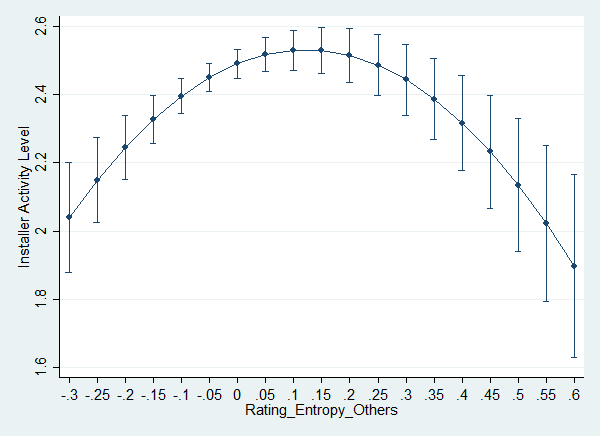
\includegraphics[width=0.7\linewidth]{marginsplot_entothers.png}
	\caption{Marginal Impact of Entropy of Reviews on Individual Level Activity}
	\label{marginsplot_ind_ent_self}
\end{figure}


\subsection{Local Markets}

\begin{figure}
	\centering
	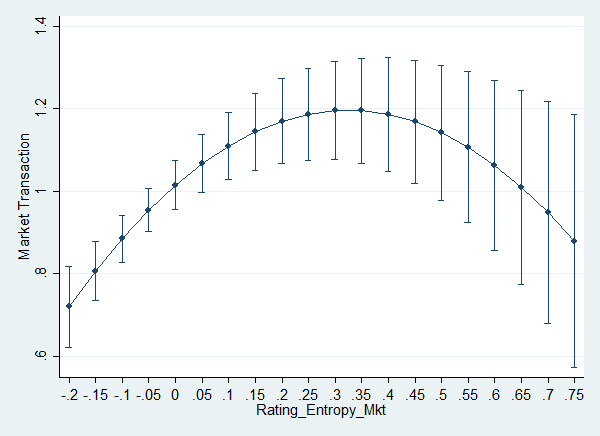
\includegraphics[width=0.7\linewidth]{marginsplot_entmkt.png}
	\caption{Marginal Impact of Market Reviews Entropy of Reviews on Market Level Activity}
	\label{marginsplot_mkt_entmkt}
\end{figure}
\begin{figure}
	\centering
	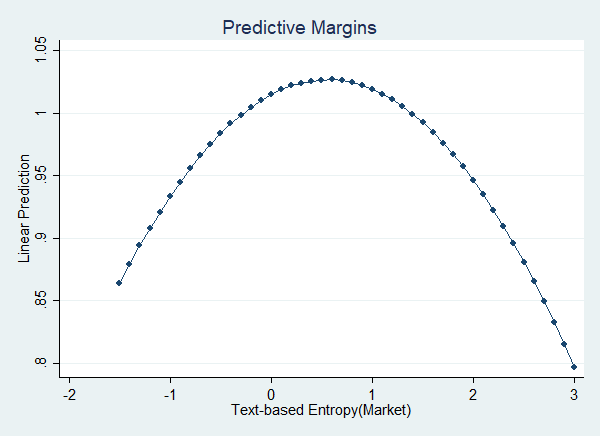
\includegraphics[width=0.7\linewidth]{marginsplot_text_ent_mkt_noci.png}
	\caption{Marginal Impact of Text-based Entropy of Reviews on Market Level Activity}
	\label{marginsplot_text_ent_mkt}
\end{figure}
We now move to discuss the ratings dispersion on total transactions on local market level. The results are presented in table \ref{reg_mkt}. Column (1) ... (4)... The estimate suggest that on the market level, reviews dispersion is directly linked to higher number of total proposals accepted, as reflected in the coefficient estimates being positive and statistically significant. We also note that the second order effect is negative as the coefficient estimates associated with the square term is negative and statistically significant. We further illustrate this point with a margins plot using coefficients generated from estimates in column X in figure \ref{marginsplot_mkt_entmkt}. \\
The relationship we found in this section is similar to what we presented earlier. The important distinction is that we are looking at local market at an entire performance unit and measuring the dispersion of ratings on the market level.
\subsection{Measures of ratings dispersion}
We replace ratings entropy with text-based dispersion and re-run both individual and market level analysis. The results are presented in table \ref{table_reg_ind_textent} and table \ref{reg_mkt_text_ent} as well as figure \ref{marginsplot_text_ent_mkt}. We observe the same type of inverse U shape for the marginal impact of text-based dispersion. This result comes at no surprise as the two measures of ratings dispersions are correlated significantly, although the magnitude of correlation isn't very high (). In table X we put in both ratings entropy and text-based reviews dispersion as presented in column (6). We found that the even after we include both  \\
% Please add the following required packages to your document preamble:
% \usepackage{booktabs}
\begin{table}
\centering
\begin{tabular}{@{}lllll@{}}
\toprule
 & (1) & (2) & (3) & (4) \\ \midrule
 & F.Tran & F.Tran & F.Tran & F.Tran \\
Entropy & 2.106*** & 2.106** & 2.195*** & 2.195*** \\
 & (0.000) & (0.003) & (0.000) & (0.000) \\
Entropy \# Entropy & -2.163*** & -2.163** & -2.309** & -2.309** \\
 & (0.000) & (0.005) & (0.001) & (0.001) \\
Market Revenue & -0.0500 & -0.0500* & -0.0471* & -0.0471* \\
 & (0.124) & (0.044) & (0.033) & (0.033) \\
Market Revenue \# Market Revenue & 0.00184 & 0.00184 & 0.00174 & 0.00174 \\
 & (0.347) & (0.179) & (0.168) & (0.168) \\
Reviews(Mkt) &  &  & -0.0818 & -0.0818 \\
 &  &  & (0.686) & (0.686) \\
Constant & 1.509 & 1.509*** & 0.805 & 0.805 \\
 & (0.175) & (0.000) & (0.395) & (0.395) \\
Observations & 754 & 754 & 736 & 736 \\
p-values in parentheses &  &  &  &  \\
="* p\textless{}0.05 & ** p\textless{}0.01 & *** p\textless{}0.001" &  &  \\ \bottomrule
\end{tabular}
\caption{Regression Market Level}
\label{reg_mkt}
\end{table}
% Please add the following required packages to your document preamble:
% \usepackage{booktabs}
\begin{table}
\centering
\begin{tabular}{@{}lllllll@{}}
\toprule
 & (1) & (2) & (3) & (4) & (5) & (6) \\ \midrule
 & F.Tran & F.Tran & F.Tran & F.Tran & F.Tran & F.Tran \\
Entropy & 2.106* & 1.682* &  &  &  & 1.528* \\
 & (0.003) & (0.001) &  &  &  & (0.001) \\
Entropy \# Entropy & -2.163* & -1.893* &  &  &  & -1.729* \\
 & (0.005) & (0.001) &  &  &  & (0.001) \\
Market Revenue & -0.0500* & -0.0300 & -0.136* & -0.0802* & -0.0802* & -0.0161 \\
 & (0.044) & (0.110) & (0.017) & (0.009) & (0.009) & (0.358) \\
Market Revenue \# Market Revenue & 0.00184 & 0.00130 & 0.00714* & 0.00446* & 0.00446* & 0.000515 \\
 & (0.179) & (0.213) & (0.029) & (0.013) & (0.013) & (0.607) \\
L.Tran &  & 0.333* &  & 0.371* & 0.371* & 0.309* \\
 &  & (0.000) &  & (0.000) & (0.000) & (0.000) \\
Text Ent &  &  & 10.20 & 7.314 &  &  \\
 &  &  & (0.241) & (0.154) &  &  \\
Text Ent\textasciicircum{}2 &  &  & -33.23 & -22.99 &  &  \\
 &  &  & (0.199) & (0.129) &  &  \\
Text Ent(Normalized) &  &  &  &  & 0.0530 & 0.0274 \\
 &  &  &  &  & (0.451) & (0.704) \\
Text Ent(Normalized)\textasciicircum{}2 &  &  &  &  & -0.0377 & -0.0298+ \\
 &  &  &  &  & (0.129) & (0.065) \\
Constant & 1.509* & 0.669* & 1.177 & 0.464 & 1.027* & 0.709* \\
 & (0.000) & (0.001) & (0.129) & (0.317) & (0.000) & (0.002) \\
Observations & 754 & 745 & 961 & 952 & 952 & 707 \\
p-values in parentheses &  &  &  &  &  &  \\
="+ p\textless{}0.10 & * p\textless{}0.05" &  &  &  &  &  \\ \bottomrule
\end{tabular}
\caption{Regression on Market Level with Text-based Entropy}
\label{reg_mkt_text_ent}
\end{table}

\section{Robustness Check}
\subsection{Endogeneity}
We now discuss the issues of endogeneity in our empirical strategies. Regarding the individual level analysis, endogeneity could occur if there are unobserved factors that is significantly correlated with ratings dispersion that is also correlated with the activity intensities.\\
Consider that we omitted a variable that captures installer professionalism or motivation, which we denote as $pro_{i,t}$. The actual function should be
\begin{equation}
ActInt_{i,m,t+1}=\delta pro_{i,t}+\beta_{1} Ent_{i,m,others,t}+\beta_{2}Ent_{i,m,others,t}^2+controls+\epsilon_{i,m,t}
\end{equation}
We argue that $pro_{it}$ would be \textit{negatively} correlated with reviews dispersion -- professional installers would be more motivated than others to deliver consistent products and services (CITE some thing).  \\

In this case, the presence of omitted variable deflated the estimates of $\beta$ (CITE ECONOMETRIC stuff). \\
\subsection{Dfferent model specifications}
- different time lag.  \\
- use CV instead of entropy(show CV is correlated with entropy but less differentiating) \\

\subsection{Robustness with local market division}
Although many similar studies used ZIP code to difine local markets(cite something from IO), we used unsupervised algorithm (OPTICS) to determine the market grouping. OPTICS algorithm requires a few parameter inputs: X, Y and Z. We used parameter XX after performing grid-search on a parameter space XXX and use Calinski-Harabasz Index to assess the appropriateness of the clustering.  \\ In addition, we used 4 digit ZIP code to define a market and the results are consistent ( INSERT RESULTS); we also use other OPTICS parameter and the results are consistent.  \\

\subsection{Dynamic Panel model}
In our main analysis we include both fixed effect for each installer to account for time invariant factors. We use a dynamic panel model to perform robustness check. The inclusion of lagged dependent variable ( Activity Intensity) aim to control for unobserved heterogeneity that may influence changes in the dependent variable and is time variant. For individual level estimation, the equation we estimate is changed into the following:
\begin{equation}
    ActInt_{i,m,t+1}=\gamma ActInt_{i,m,t-1}+Ent_{i,m,others,t}+Ent_{i,m,others,t}^2+
    controls+\epsilon_{i,m,t}
\end{equation}

\begin{equation}
    ActInt_{im,t+1}=\gamma Ent_{im,t-1}+\beta_{3}+\beta_{4} Ent_{i,self,t}+\beta_{5}Ent_{i,self,t}^2+
   Controls+\epsilon_{imt}
   \label{model_ind_dyn_1}
\end{equation}

\begin{equation}
    ActInt_{im,t+1}=\gamma Ent_{im,t-1}+\beta_{6}+\beta_{7} Ent_{i,self,t}+\beta_{8}Ent_{i,self,t}^2+\beta_{9}Ent_{im,others}+\beta_{10}Ent_{im,self,t}^2+
   Controls+\epsilon_{imt}
   \label{model_ind_dyn_2}
\end{equation}
We expect $\gamma$ estimates to be positive. The results are still consistent as the $\beta$ coefficients associated with $Ent_{others}$($Ent_{others}^2$) are still positive (negative) as presented in table \ref{rob_addlag} and \ref{rob_addlag_withentself}.

Likewise, we modify the market level model to include a lagged dependent variable $MarketActivity_{m,t-1})$
\begin{equation}
    MarketActivity_{m,t+1}=\gamma MarketActivity_{m,t-1}+\beta Ent_{m,t}+\beta Ent_{m,t}^2+Controls+\epsilon_{mt}
\end{equation}
and the results, presented in table \ref{rob_addlag_mkt}, are still consistent.
% Please add the following required packages to your document preamble:
% \usepackage{booktabs}
\begin{table}
\centering
\begin{tabular}{@{}lcccc@{}}
\toprule
 & (1) & (2) & (3) & (4) \\ \midrule
 & F.Activity & F.Activity & F.Activity & F.Activity \\
Avg & -0.655 & -0.655 & -0.508 & -0.508 \\
 & (0.345) & (0.283) & (0.204) & (0.211) \\
Avg $^2$ & 0.0471 & 0.0471 & 0.0375 & 0.0375 \\
 & (0.660) & (0.614) & (0.572) & (0.563) \\
Reviews Count & 0.0480* & 0.0480* & 0.0273* & 0.0273* \\
 & (0.000) & (0.000) & (0.000) & (0.001) \\
Avg(Others) & -0.0285 & -0.0285 & -0.0491 & -0.0491 \\
 & (0.873) & (0.876) & (0.754) & (0.717) \\
Entropy Others & 1.762* & 1.762* & 1.485* & 1.485* \\
 & (0.020) & (0.012) & (0.009) & (0.006) \\
Experience & 0.212* & 0.212* & 0.141+ & 0.141+ \\
 & (0.021) & (0.018) & (0.083) & (0.056) \\
Price Diff & 0.0861 & 0.0861 & 0.0120 & 0.0120 \\
 & (0.569) & (0.557) & (0.908) & (0.913) \\
Market Revenue & -0.0169+ & -0.0169* & -0.0136+ & -0.0136* \\
 & (0.074) & (0.023) & (0.100) & (0.024) \\
Entropy Others  $^2$ & -2.626* & -2.626* & -2.148* & -2.148* \\
 & (0.001) & (0.005) & (0.000) & (0.003) \\
L.Activity &  &  & 0.324* & 0.324* \\
 &  &  & (0.000) & (0.000) \\
Constant & 4.062* & 4.062* & 3.128* & 3.128* \\
 & (0.004) & (0.004) & (0.004) & (0.003) \\
Observations & 4190 & 4190 & 4047 & 4047 \\
p-values in parentheses &  &  &  &  \\
="+ p\textless{}0.10 & * p\textless{}0.05" &  &  &  \\ \bottomrule
\end{tabular}
\caption{Robustness Check Add Lagged DV}
\label{rob_addlag}
\end{table}
% Please add the following required packages to your document preamble:
% \usepackage{booktabs}
% \usepackage{graphicx}
\begin{table}
\centering
\begin{tabular}{@{}lcccc@{}}
\toprule
 & (1) & (2) & (3) & (4) \\ \midrule
 & F.Activity & F.Activity & F.Activity & F.Activity \\
Avg & -1.170+ & -0.862+ & -1.155+ & -0.850+ \\
 & (0.068) & (0.054) & (0.060) & (0.055) \\
Avg $^2$ & 0.130 & 0.0944 & 0.129 & 0.0926 \\
 & (0.180) & (0.203) & (0.170) & (0.207) \\
Reviews Count & 0.0452* & 0.0254* & 0.0423* & 0.0230* \\
 & (0.000) & (0.001) & (0.000) & (0.002) \\
Avg(Others) & -0.0310 & -0.0611 & -0.0273 & -0.0435 \\
 & (0.857) & (0.672) & (0.887) & (0.795) \\
Experience & 0.211* & 0.141+ & 0.207* & 0.139+ \\
 & (0.019) & (0.077) & (0.023) & (0.086) \\
Price Diff & 0.0863 & 0.0160 & 0.0928 & 0.0188 \\
 & (0.554) & (0.875) & (0.516) & (0.849) \\
Market Revenue & -0.0163 & -0.0131 & -0.0160 & -0.0130 \\
 & (0.107) & (0.135) & (0.109) & (0.134) \\
Entropy Own & 2.616* & 2.009* & 2.676* & 2.061* \\
 & (0.006) & (0.008) & (0.004) & (0.004) \\
Entropy Own $^2$ & -3.090* & -2.425* & -3.301* & -2.602* \\
 & (0.042) & (0.024) & (0.020) & (0.007) \\
L.Activity &  & 0.322* &  & 0.320* \\
 &  & (0.000) &  & (0.000) \\
Entropy Others &  &  & 1.740* & 1.478* \\
 &  &  & (0.022) & (0.009) \\
Entropy Others$^2$ &  &  & -2.674* & -2.204* \\
 &  &  & (0.001) & (0.000) \\
Constant & 4.698* & 3.649* & 4.519* & 3.437* \\
 & (0.001) & (0.001) & (0.002) & (0.003) \\
Observations & 4190 & 4047 & 4190 & 4047 \\
p-values in parentheses &  &  &  &  \\
="+ p\textless{}0.10 & * p\textless{}0.05" &  &  &  \\ \bottomrule
\end{tabular}%
\caption{Robustness Check with Lagged Variable and Own Entropy}
\label{rob_addlag_withentself}
\end{table}
% Please add the following required packages to your document preamble:
% \usepackage{booktabs}
\begin{table}
\centering
\begin{tabular}{@{}lcccc@{}}
\toprule
 & (1) & (2) & (3) & (4) \\ \midrule
 & F.Tran & F.Tran & F.Tran & F.Tran \\
Entropy & 2.106* & 2.106* & 1.682* & 1.682* \\
 & (0.000) & (0.003) & (0.000) & (0.001) \\
Entropy $^2$ & -2.163* & -2.163* & -1.893* & -1.893* \\
 & (0.000) & (0.005) & (0.000) & (0.001) \\
Market Revenue & -0.0500 & -0.0500* & -0.0300 & -0.0300 \\
 & (0.124) & (0.044) & (0.332) & (0.110) \\
Market Revenue $^2$ & 0.00184 & 0.00184 & 0.00130 & 0.00130 \\
 & (0.347) & (0.179) & (0.483) & (0.213) \\
L.Tran &  &  & 0.333* & 0.333* \\
 &  &  & (0.000) & (0.000) \\
Constant & 1.509 & 1.509* & 0.669 & 0.669* \\
 & (0.175) & (0.000) & (0.527) & (0.001) \\
Observations & 754 & 754 & 745 & 745 \\
p-values in parentheses &  &  &  &  \\
="+ p\textless{}0.10 & * p\textless{}0.05" &  &  &  \\ \bottomrule
\end{tabular}
\caption{Robustness Check Market Level Add Lagged DV}
\label{rob_addlag_mkt}
\end{table}

\subsection{Excluding Inactive Installers}
Although we do not explicly model the process of installers exiting platform, we are aware of its potential to drive resutls. We ran a robustness check excluding installers that have been inactive for two month ( making 0 proposals), with results presented in table \ref{rob_exclude_inactive}. The first two columns are results excluding these said installers ( cluster standard errors on market level - column (1); individual level - column (2)) . The results are virtually unchanged, especially on the independent variable of interests.
% Please add the following required packages to your document preamble:
% \usepackage{booktabs}
\begin{table}
\centering
\begin{tabular}{@{}lcccc@{}}
\toprule
 & (1) & (2) & (3) & (4) \\ \midrule
 & F.Activity & F.Activity & F.Activity & F.Activity \\
Avg & -0.532 & -0.532 & -0.655 & -0.655 \\
 & (0.270) & (0.265) & (0.345) & (0.283) \\
Avg \# Avg & 0.0448 & 0.0448 & 0.0471 & 0.0471 \\
 & (0.543) & (0.530) & (0.660) & (0.614) \\
Reviews Count & 0.0485* & 0.0485* & 0.0480* & 0.0480* \\
 & (0.000) & (0.000) & (0.000) & (0.000) \\
Avg(Others) & 0.00612 & 0.00612 & -0.0285 & -0.0285 \\
 & (0.958) & (0.967) & (0.873) & (0.876) \\
Ent Others & 1.396* & 1.396* & 1.762* & 1.762* \\
 & (0.018) & (0.021) & (0.020) & (0.012) \\
Experience & 0.133+ & 0.133+ & 0.212* & 0.212* \\
 & (0.086) & (0.075) & (0.021) & (0.018) \\
Price Diff & 0.206 & 0.206 & 0.0861 & 0.0861 \\
 & (0.182) & (0.118) & (0.569) & (0.557) \\
Market Revenue & -0.00619 & -0.00619 & -0.0169+ & -0.0169* \\
 & (0.424) & (0.330) & (0.074) & (0.023) \\
Ent Others \# Ent Others & -2.252* & -2.252* & -2.626* & -2.626* \\
 & (0.000) & (0.007) & (0.001) & (0.005) \\
Constant & 3.745* & 3.745* & 4.062* & 4.062* \\
 & (0.000) & (0.001) & (0.004) & (0.004) \\
Observations & 3465 & 3465 & 4190 & 4190 \\
p-values in parentheses &  &  &  &  \\
="+ p\textless{}0.10 & * p\textless{}0.05" &  &  &  \\ \bottomrule
\end{tabular}
\caption{Robustness Check Excluding Inactive Installers}
\label{rob_exclude_inactive}
\end{table}
\clearpage
\begin{APPENDIX}{Tables and Figures}




\end{APPENDIX}
\clearpage
% Appendix here
% Options are (1) APPENDIX (with or without general title) or
%             (2) APPENDICES (if it has more than one unrelated sections)
% Outcomment the appropriate case if necessary
%
% \begin{APPENDIX}{<Title of the Appendix>}
% \end{APPENDIX}
%
%   or
%
% \begin{APPENDICES}
% \section{<Title of Section A>}
% \section{<Title of Section B>}
% etc
% \end{APPENDICES}


% Acknowledgments here
\ACKNOWLEDGMENT{ .}


% References here (outcomment the appropriate case)

% CASE 1: BiBTeX used to constantly update the references
%   (while the paper is being written).
%\bibliographystyle{informs2014} % outcomment this and next line in Case 1
%\bibliography{<your bib file(s)>} % if more than one, comma separated

% CASE 2: BiBTeX used to generate mypaper.bbl (to be further fine tuned)
%\input{mypaper.bbl} % outcomment this line in Case 2

%If you don't use BiBTex, you can manually itemize references as shown below.


\bibliographystyle{informs2014} % outcomment this and next line in Case 1
\bibliography{solarlits} % if more than one, comma separated


%%%%%%%%%%%%%%%%%
\end{document}
%%%%%%%%%%%%%%%%%

